\documentclass[conference]{IEEEtran}
\renewcommand\IEEEkeywordsname{keywords}
\usepackage{graphicx}
\usepackage{epstopdf}
\usepackage{float}
\usepackage{amssymb}
\usepackage{multirow}
\usepackage[english]{babel}
\usepackage{algorithmic,algorithm}
\renewcommand{\algorithmicrequire}{\textbf{Input:}}
\renewcommand{\algorithmicensure}{\textbf{Output:}}
\usepackage{enumerate}
\usepackage{lipsum}% http://ctan.org/pkg/lipsum
\hyphenation{op-tical net-works semi-conduc-tor}
\usepackage{booktabs}
\usepackage{amsmath}
\usepackage[smallscripts]{moresize}
%\usepackage[numbers,sort&compress]{natbib}
\usepackage[numbers,sort]{natbib}
\usepackage[most]{tcolorbox}
%\usepackage{ctable}

\begin{document}

\title{Combining Deep Learning and Computer Vision for Multiclass Disease Detection in Potato, Tomato, and Bell Pepper Plants}
%%%%%%%%%%%%%%%%%%%%%%%%%%%%%%%%%%%%%%%
% \author{\IEEEauthorblockN{Utpal Kant Singh, Rajnish Kumar, Saurabh Kumar, Shibasish Kar, Santos Kumar Baliarsingh}

% \IEEEauthorblockA{School of Computer Engineering,
% KIIT Deemed to be University, Bhubaneswar, 751024, India}
% \{20051117, 2005118, 20051096, 2005335, santos.baliarsinghfcs\}@kiit.ac.in
% }
%%%%%%%%%%%%%%%%%%%%%%%%%%%%%%%%%%%%
\author{\IEEEauthorblockN{Utpal Kant Singh}
\IEEEauthorblockA{School of Computer Engineering\\
KIIT Deemed to be University,\\ Bhubaneswar, India 751024\\
Email: utpalkant.4855@gmail.com}
\and
\IEEEauthorblockN{Vishal R. Satpute}
\IEEEauthorblockA{Department of Electronics and \\Communication Engineering\\
VNIT, Nagpur, India 440010\\
Email: vrsatpute@ece.vnit.ac.in}
}
%%%%%%%%%%%%%%%%%%%%%%%%%%%%%%%%%%%%%%%%%%%%%


\maketitle

\begin{abstract}

Tomato, potato, and bell pepper are important crops in India, benefiting from the country's tropical climate. However, various factors, including climatic conditions, can adversely affect their growth and overall production. Plant diseases pose a significant threat to these crops, leading to substantial financial losses. Traditional methods of disease detection in tomato, potato, and bell pepper plants have proven to be inefficient and time-consuming. Early identification of diseases is crucial for effective disease management. This study investigates the potential of deep learning techniques, particularly convolutional neural networks (CNNs), combined with computer vision technology, for the accurate diagnosis of diseases in tomato, potato, and bell pepper plant leaves. The results demonstrate the effectiveness of the proposed approach, achieving an impressive average accuracy of 95\% in classifying leaf diseases in these crops. \\

 
\end{abstract}


\begin{IEEEkeywords}
Deep Learning, Machine Learning, Potato Leaf Disease Detection, Convolutional Neural Network, 
\end{IEEEkeywords}
 
\IEEEpeerreviewmaketitle



\section{Introduction}



\subsection{Motivation}
The cultivation of diverse crops, including tomato, potato, and bell pepper, is vital for meeting the agricultural needs of the Indian economy. However, these crops are susceptible to various diseases, which can significantly impact crop yield and quality. Early detection and treatment of these diseases are crucial for safeguarding the livelihoods of farmers. Traditional disease management approaches often rely on the use of pesticides, which have detrimental effects on the environment. Therefore, early disease detection promotes sustainable agricultural practices by reducing the reliance on chemical interventions. Furthermore, certain diseases affecting tomato, potato, and bell pepper plants can pose risks to human health through contaminated produce or exposure to toxins. Timely diagnosis and treatment of these diseases can help mitigate these risks. Automated methods for accurate and reliable disease detection in tomato, potato, and bell pepper plant leaves are essential, as manual inspection methods are costly and resource-intensive. \\ 

The domains of object identification and picture classification have seen a considerable revolution since the introduction of CNNs. The use of CNNs in disease detection has the potential to completely change how illnesses that afflict tomato, potato, and bell pepper plants are identified and treated. Early disease identification made possible by CNNs can significantly reduce crop losses and increase output as a whole. By making correct diagnoses, CNNs eliminate the need for human specialists and cut down on the possibility of mistakes occurring during visual examinations. Additionally, CNNs can drastically save costs and turnaround times when used in automated illness identification, especially in areas with limited resources. This easily available and reasonably priced technology can help farmers get past knowledge and resource limitations, which will improve the results of growing tomato, potato, and bell pepper plants.\\

The expenses and turnaround times associated with conventional diagnostic techniques can be greatly reduced by adopting CNNs for automated disease diagnosis. This is particularly crucial in developing nations where there are little resources and specialists available for correctly diagnosing and treating plant diseases. For farmers, CNNs improve accessibility and affordability by offering a more accessible and cost-effective means of diagnosis.


\subsection{Contributions}
\begin{itemize}
    \item A system for classifying illnesses affecting potato leaves is created using a convolutional neural network (CNN) architecture based on deep learning. The main goal of the system is to accurately and correctly classify the many diseases that impact potato plants.
    \item The CNN model, which is suggested for the classification of potato plant leaf diseases, outperforms more sophisticated models in testing and comparisons, demonstrating its amazing performance.
    \item Experiments using a publicly accessible dataset of potato plant leaf diseases are used to assess the efficacy and usefulness of the proposed CNN-based technique. The findings of the experiment provide vital details on the possible uses of the suggested approach for illness diagnosis and classification in agriculture.\\
\end{itemize}
 
The goal of this study is to assess how well CNNs work in automatically spotting illnesses in the leaves of bell pepper, potato, and tomato plants. The results of this study might be used to improve disease detection methods for tomato, potato, and bell pepper crops, which would be of enormous use to the agricultural community and the world's food supply chain.

\section{Related Works}
Although bell peppers are a popular and nutritious crop, they are susceptible to various diseases that can lead to significant decreases in crop yield if not promptly identified and addressed. To address this issue, researchers have begun automating the detection and categorization of diseases in tomato, potato, and bell pepper plant leaves using advanced deep learning techniques, specifically CNNs.\\

Early detection and effective management of diseases in potato leaves are crucial in minimizing their impact. Asif et al. \cite{9316021} propose a model that utilizes image processing techniques for precise identification and detection of diseases in potato leaves. Among various machine learning algorithms, the Convolutional Neural Network (CNN) model is chosen for its exceptional performance in tasks related to image classification. The study incorporates five different algorithms, including AlexNet, VggNet, ResNet, LeNet, and a Sequential model developed by the authors. The model is trained using a diverse dataset containing both healthy and diseased leaf images, enabling the differentiation between normal and abnormal aspects of potato leaves. Through the implemented algorithm, the model achieves an impressive precision of 97\% in accurately classifying potato plant leaves as either diseased or healthy. This research underscores the significance of disease detection in potato plants and highlights the efficacy of the proposed CNN-based model in precisely identifying diseases in potato leaves.\\


In order to promote sustainable agricultural development, it is crucial to conduct research in the field of plant disease diagnosis, capitalizing on advancements in agricultural technology and artificial intelligence. Diseases such as early blight and late blight have a significant impact on potato crops, and manually identifying these leaf diseases can be a challenging and time-consuming task. Early and automated detection of these diseases can greatly enhance potato crop production. Previous studies have proposed various models for disease detection. In this particular study \cite{9121067}, the authors propose a model that utilizes pre-trained models like VGG19 and fine-tuning through transfer learning to extract relevant features from the dataset. Multiple classifiers are employed, and logistic regression demonstrates superior performance, achieving a high classification accuracy of 97.8\% on the test dataset. This research contributes to the advancement of efficient disease detection systems for potatoes, ultimately leading to improved crop productivity and quality.\\

The Plant Disease Detection Neural Network (PDDNN), a unique CNN model created by Hari et al. \cite{8899748} for their study and optimised for crop leaf image analysis, was introduced. The PDDNN has 16 layers and, in order to improve performance, uses various filters, dropout layers, and max pool layers. An outstanding accuracy rate of 86\% was attained by the PDDNN by using a bigger dataset of 14,810 photos. Notably, the PDDNN outperformed the Mobilenet 50 network by around 7\% in terms of accuracy, demonstrating higher performance in comparison. This study emphasises the PDDNN model's usefulness and superiority over other available models for plant disease identification.\\

Potato crops are significantly impacted by diseases, affecting both their quality and yield. Timely detection and accurate classification of these diseases are crucial to prevent further deterioration and minimize losses. Leaf conditions provide valuable insights for identifying different diseases in potato plants. This study \cite{9231784} presents a classification system that effectively categorizes four types of potato plant diseases based on leaf conditions. To develop the system, deep learning techniques utilizing the VGG16 and VGG19 convolutional neural network architectures are employed. The experimental results demonstrate the effectiveness of the deep neural network approach, achieving an average classification accuracy of 91\% in potato disease identification. This research contributes to the field by providing a reliable and precise method for early disease detection, enabling prompt intervention and improved crop management practices.\\

Traditional machine learning methods often struggle to generalize effectively across different crop species and diseases due to their reliance on specific regional datasets for training and testing. However, in this research \cite{electronics10172064}, a multi-level deep learning model is proposed to address this challenge in the identification of potato leaf diseases. The model incorporates YOLOv5 image segmentation techniques to isolate potato leaves from plant images, followed by a novel convolutional neural network specifically designed to detect early blight and late blight diseases in potato leaf images. To evaluate the model's performance, a dataset comprising 4062 images collected from the Central Punjab region of Pakistan is used, resulting in an impressive accuracy rate of 99.75\%. Furthermore, the model is compared to state-of-the-art approaches, demonstrating superior accuracy and computational efficiency. This research significantly contributes to the field of potato leaf disease detection by providing a robust and accurate solution for early diagnosis and effective management of potato crops.\\

Effectively managing and controlling diseases in potato leaf crops is vital for farmers to increase their productivity and minimize agricultural losses. The automation of disease identification can provide valuable support to farmers in their disease control efforts. In this research \cite{9181312}, a specialized Convolutional Neural Network (CNN) architecture is introduced for the detection of potato diseases. The CNN framework incorporates image processing techniques to generate a training dataset. The model is optimized using the Adam optimizer and cross entropy analysis, with the softmax function utilized for final evaluation. The architecture is designed to achieve high accuracy while minimizing resource usage. Experimental results demonstrate the effectiveness of the proposed model, achieving a disease detection accuracy of 99\% with a parameter usage of 10,089,219. This study offers a robust and accurate approach for potato disease detection, enabling timely intervention and improved disease management practices in the agricultural sector.\\


The research conducted by Afonso et al. \cite{AFONSO20196} aims to utilize deep learning techniques for the detection of blackleg disease in potato plants. The study trains two deep convolutional neural networks, including ResNet18, using RGB images that consist of both healthy and diseased plants. The experimental results demonstrate the effectiveness of the ResNet18 network, achieving a precision rate of 95\% and a recall rate of 91\% for identifying the disease. These findings highlight the potential of convolutional neural networks as a valuable tool for early detection and effective management of blackleg disease in potato plants. This technology can facilitate proactive intervention and improve disease management strategies.\\

 Deep learning and computer vision techniques, specifically Convolutional Neural Networks (CNN), have proven to be effective in detecting plant diseases. In this research paper \cite{sharma2022plant}, the authors propose a CNN model for classifying rice and potato leaf diseases. The dataset consists of images of rice leaves affected by bacterial blight, blast, brown spot, and tungro diseases, as well as potato leaf images with healthy leaves, early blight, and late blight diseases. The CNN model achieves impressive levels of accuracy, with a classification accuracy of 99.58\% for rice leaf diseases and 97.66\% for potato leaf diseases. These results demonstrate the superiority of the CNN model compared to other machine learning classifiers such as Support Vector Machine, K-Nearest Neighbors, Decision Tree, and Random Forest, in the field of image-based plant disease identification.\\

Timely detection and immediate intervention are crucial for preventing the spread of diseases in plants. However, growers often struggle to identify diseases on their plants, underscoring the need for an effective and precise identification model. Image processing techniques play a crucial role in analyzing digital data, especially in the context of plant disease identification, which can be challenging due to the complexity of the data. In their study, Kapoor et al. \cite{kapoor2023bell} focus on employing two deep learning models, namely AlexNet and VGG16, for the identification of leaf diseases in bell pepper plants. The experimental results demonstrate promising levels of accuracy, with AlexNet achieving 97.80\% accuracy and VGG16 achieving an even higher accuracy of 99.38\%. These findings highlight the potential of deep learning models in accurately detecting and classifying leaf diseases in bell pepper plants, providing valuable insights for disease management and prevention strategies.\\

The agricultural sector plays a critical role in the economy, and accurately identifying diseases in plants is essential for maintaining optimal crop yields. However, manual monitoring of plants for disease detection is time-consuming and requires significant labor. To address this challenge, Mustafa et al. \cite{mustafa2023pepper} employ image processing techniques, including Convolutional Neural Networks (CNNs), in agriculture. Their study presents a novel five-layered CNN model specifically designed for automatic plant disease detection using leaf images. To improve the training process, a large dataset of 20,000 augmented images is generated. The experimental results demonstrate the effectiveness of the proposed optimized CNN model, achieving an impressive accuracy rate of 99.99\% in distinguishing between healthy and bacterial-infected bell pepper plant leaves. With its robust performance, the optimized CNN model holds promising potential as an early warning system for disease identification in real cultivation environments.\\

Bacterial spot disease poses a significant threat to the cultivation of Bell Pepper crops, leading to substantial damage to the plants and their fruits. Conventional methods of disease detection, such as laboratory diagnosis and visual inspection, have limitations in terms of both time and accuracy. To overcome these limitations, Prateek et al. \cite{9565945} investigate the application of Convolutional Neural Network (CNN) architectures, including InceptionV3, ResNet50, and VGG16, for the identification of bacterial leaf spot disease in Bell Pepper plants. The models are trained and evaluated using a dataset consisting of diseased and healthy leaves from the Plant Village dataset, and image augmentation techniques are employed to enhance the performance of the models. The models are further optimized by adjusting parameters such as learning rates, batch size, and epochs, resulting in high accuracies. Among the models, VGG16 achieves the best performance, with an accuracy of 99.72\% and an AUC of 0.998. ResNet50 follows with an accuracy of 99.31\% and an AUC of 0.994, while InceptionV3 achieves an accuracy of 95.77\% and an AUC of 0.953.\\


In summary, the application of convolutional neural networks (CNNs) has shown promising results in automatically identifying and classifying diseases in tomato, potato, and bell pepper plant leaves. Several studies have achieved significant levels of accuracy, highlighting the potential of this approach. Ongoing research aims to enhance CNN performance through techniques such as transfer learning, SVM classifiers, and the incorporation of additional visual information. These advancements in CNN-based disease classification have the potential to greatly impact crop management practices and mitigate losses caused by diseases in tomato, potato, and bell pepper plants.

% \begin{itemize}
%   \item \textit{Map phase}: In this phase, the input data is processed locally and an input key-value pair is created. A map function is applied to the local data by each node and consequently, the output is sent to a temporary storage with a key-value pair.
% \end{itemize}


% \begin{itemize}
%   \item \textit{Reduce phase}: This phase is carried out in three phases namely, fetch, sort, and reduce. In the first phase, it fetches local copies of all the assigned map results from the map worker nodes. In the sort phase, it merges the copied results into a single sorted set of key-value pairs. In the last phase, the reduce method is invoked for each key, with  records combined into an iterable collection. Then the final result is written and saved to the output destination HDFS. 
% \end{itemize}   
% Figure~\ref{fig:hadoop} shows the architecture and life cycle of MapReduce.




% \begin{figure*}
% \centering
% \includegraphics[width=\textwidth{flowchart2}
% \caption{The flow diagram of the proposed anomaly detection approach}
% \label{fig:architecture}
% \end{figure*}



\section{Proposed Work}
The proposed study aims to utilize convolutional neural networks (CNNs) for the detection and classification of diseases affecting tomato, potato, and bell pepper plant leaves. These crops are prone to various diseases that can significantly impact crop yields if not promptly identified and treated. Conventional methods relying on manual examination by experts are time-consuming, subjective, and prone to errors. Therefore, there is a need for automated systems that can efficiently and accurately identify diseases in tomato, potato, and bell pepper plant leaves through image-based analysis.

The suggested model offers various advantages over earlier techniques used in the leaves of tomato, potato, and bell pepper plants for the same objective. By using cutting-edge methods like transfer learning, data augmentation, and complex CNN architectures, it improves the ability to extract important information from photos of these plant leaves. This development improves illness classification accuracy and lessens the possibility of incorrect diagnosis.

To address the flaws of past models, the suggested model takes use of a larger and more diversified collection of images of bell pepper plant leaves. The addition of a greater variety of sickness patterns improves the model's ability to generalise to new and unstudied data. As a result, the model operates more effectively in novel circumstances and is more flexible to circumstances that it has never seen before.

One of the most important aspects of the suggested model is the efficient use of computational resources. The model employs optimised CNN architectures and methods to deliver astounding accuracy while reducing processing requirements and inference time. As a result, it is particularly helpful for real-time applications for sickness detection and categorization in scenarios with constrained resources.


The proposed model offers a reliable and practical approach that surpasses the current models in accuracy and dependability. It presents a valuable solution for automated disease identification in tomato, potato, and bell pepper plant leaves, aiming to prevent crop losses and ensure stable production. By utilizing this technology, effective management strategies can be implemented.

Figure~\ref{fig: Figure 1} demonstrates the division of the dataset into multiple sets for training and testing purposes. A subset of the testing set is allocated for validation. The model undergoes improvement by adjusting its hyperparameters based on the validation data, following the training process with the training data. The training procedure concludes when the desired number of epochs is achieved. Ultimately, the model's effectiveness and performance are evaluated using the test data.


\begin{figure}[H]
 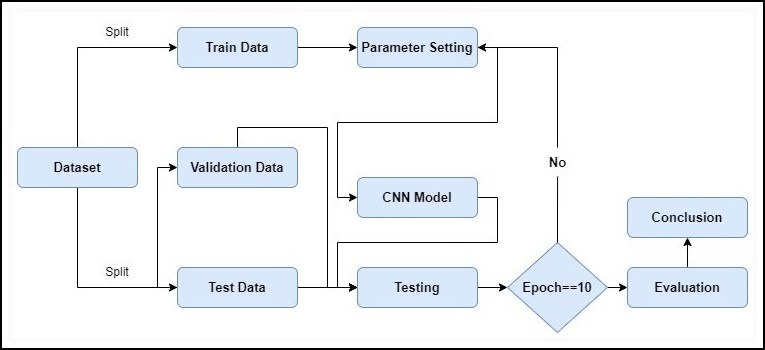
\includegraphics[width=8.8cm, height=4cm]{Tomato Final Flowchart.jpg}
\caption{Flowchart of the proposed work}
\label{fig: Figure 1}
\end{figure}

\subsection{Data Pre-Processing}
Since the PlantVillage collection already includes pre-processed photographs with little to no distortion, normalising the photos doesn't take any further work.\\
Additionally, data augmentation techniques including rotation, flipping, and zooming were applied to the training set in order to increase the dataset size and strengthen the robustness of the CNN model.\\
Overall, the information included in this classification of potato leaf diseases is vast, diverse, and suggestive of a wide range of potato ailments.





% \subsection{Temporal Attention module}
% Inspired by the various attention techniques~\cite{.....}, we employ a temporal attention module to capture temporal dependencies among snippets. After that, the attention scores are multiplied with the feature vectors to detect anomaly events. Thus, the temporal attention module allows the network to concentrate on the more important snippets.


\subsection{CNN - Convolutional Neural Network}

Convolutional neural networks (CNNs) are an advanced form of neural network that are mostly used for processing visual input like photos and videos. Due to their many levels, they have proven to be quite useful in jobs requiring image and video processing. Convolutional layers in the model use trainable filters to extract important data from the input images. The computational cost of these obtained attributes is decreased by pooling layers. By translating the returned properties to the relevant output classes, fully linked layers are used to appropriately categorise the input. Through its use in object identification, semantic segmentation, and picture classification, CNNs have revolutionised computer vision. Utilising CNNs to automatically identify and categorise plant diseases, particularly those that impact tomato leaves, has been the subject of recent study. Customised versions of the ResNet architecture have been shown to be the most accurate when compared to well-known deep learning architectures like AlexNet and GoogleNet.\\


The ResNet50 architecture, initially proposed by Zhang et al. in a 2015 study \cite{Zhang_2021_WACV}, served as the foundation for our deep neural network model.

The fundamental idea behind ResNet is the establishment of residual connections, which enable unrestricted information flow between various network layers. This is done by creating skip connections, which provide a faster information flow by connecting one layer's input to another layer's output.\\

By utilising skip connections, ResNet effectively overcomes the problem of disappearing gradients frequently seen in deep neural networks. These connections allow for more uniform gradient flow during backpropagation, enhancing the efficacy of deep network training. ResNet makes it possible for very deep networks to be trained more effectively, which enhances gradient propagation.\\

ResNet is a well-liked, widely used architecture that may take many different shapes. Among these types, ResNet50 stands out thanks to its incredible 50-layer structure. ResNet50 has demonstrated exceptional performance in a range of visual computing tasks, including scene segmentation, object tracking, and image recognition. Its exceptional abilities have lifted the bar and led to significant advancements across a range of areas.

\section{Experiment}
\subsection{Dataset}
The publicly accessible PlantVillage dataset's 54,000 labelled photos from 14 distinct crop kinds were utilised in the study. There were 20,639  tomato, potato and bell pepper leaf photos in total, each with a pixel size of 256. 15 classes were created from the images of tomato, potato, and bell pepper leaves, with 3 displaying healthy leaves and the other 12 indicating various disease stages. The dataset was split into three subsets for easier analysis: the training set, which contained 70\% of the images; the test set, which contained 15\% of the images; and the validation set, which also contained 15\% of the images. As shown in Figure~\ref{fig: Figure 2}, each image in the dataset was taken in the JPEG format and represented using the RGB colour space.



 \begin{figure}[H]
 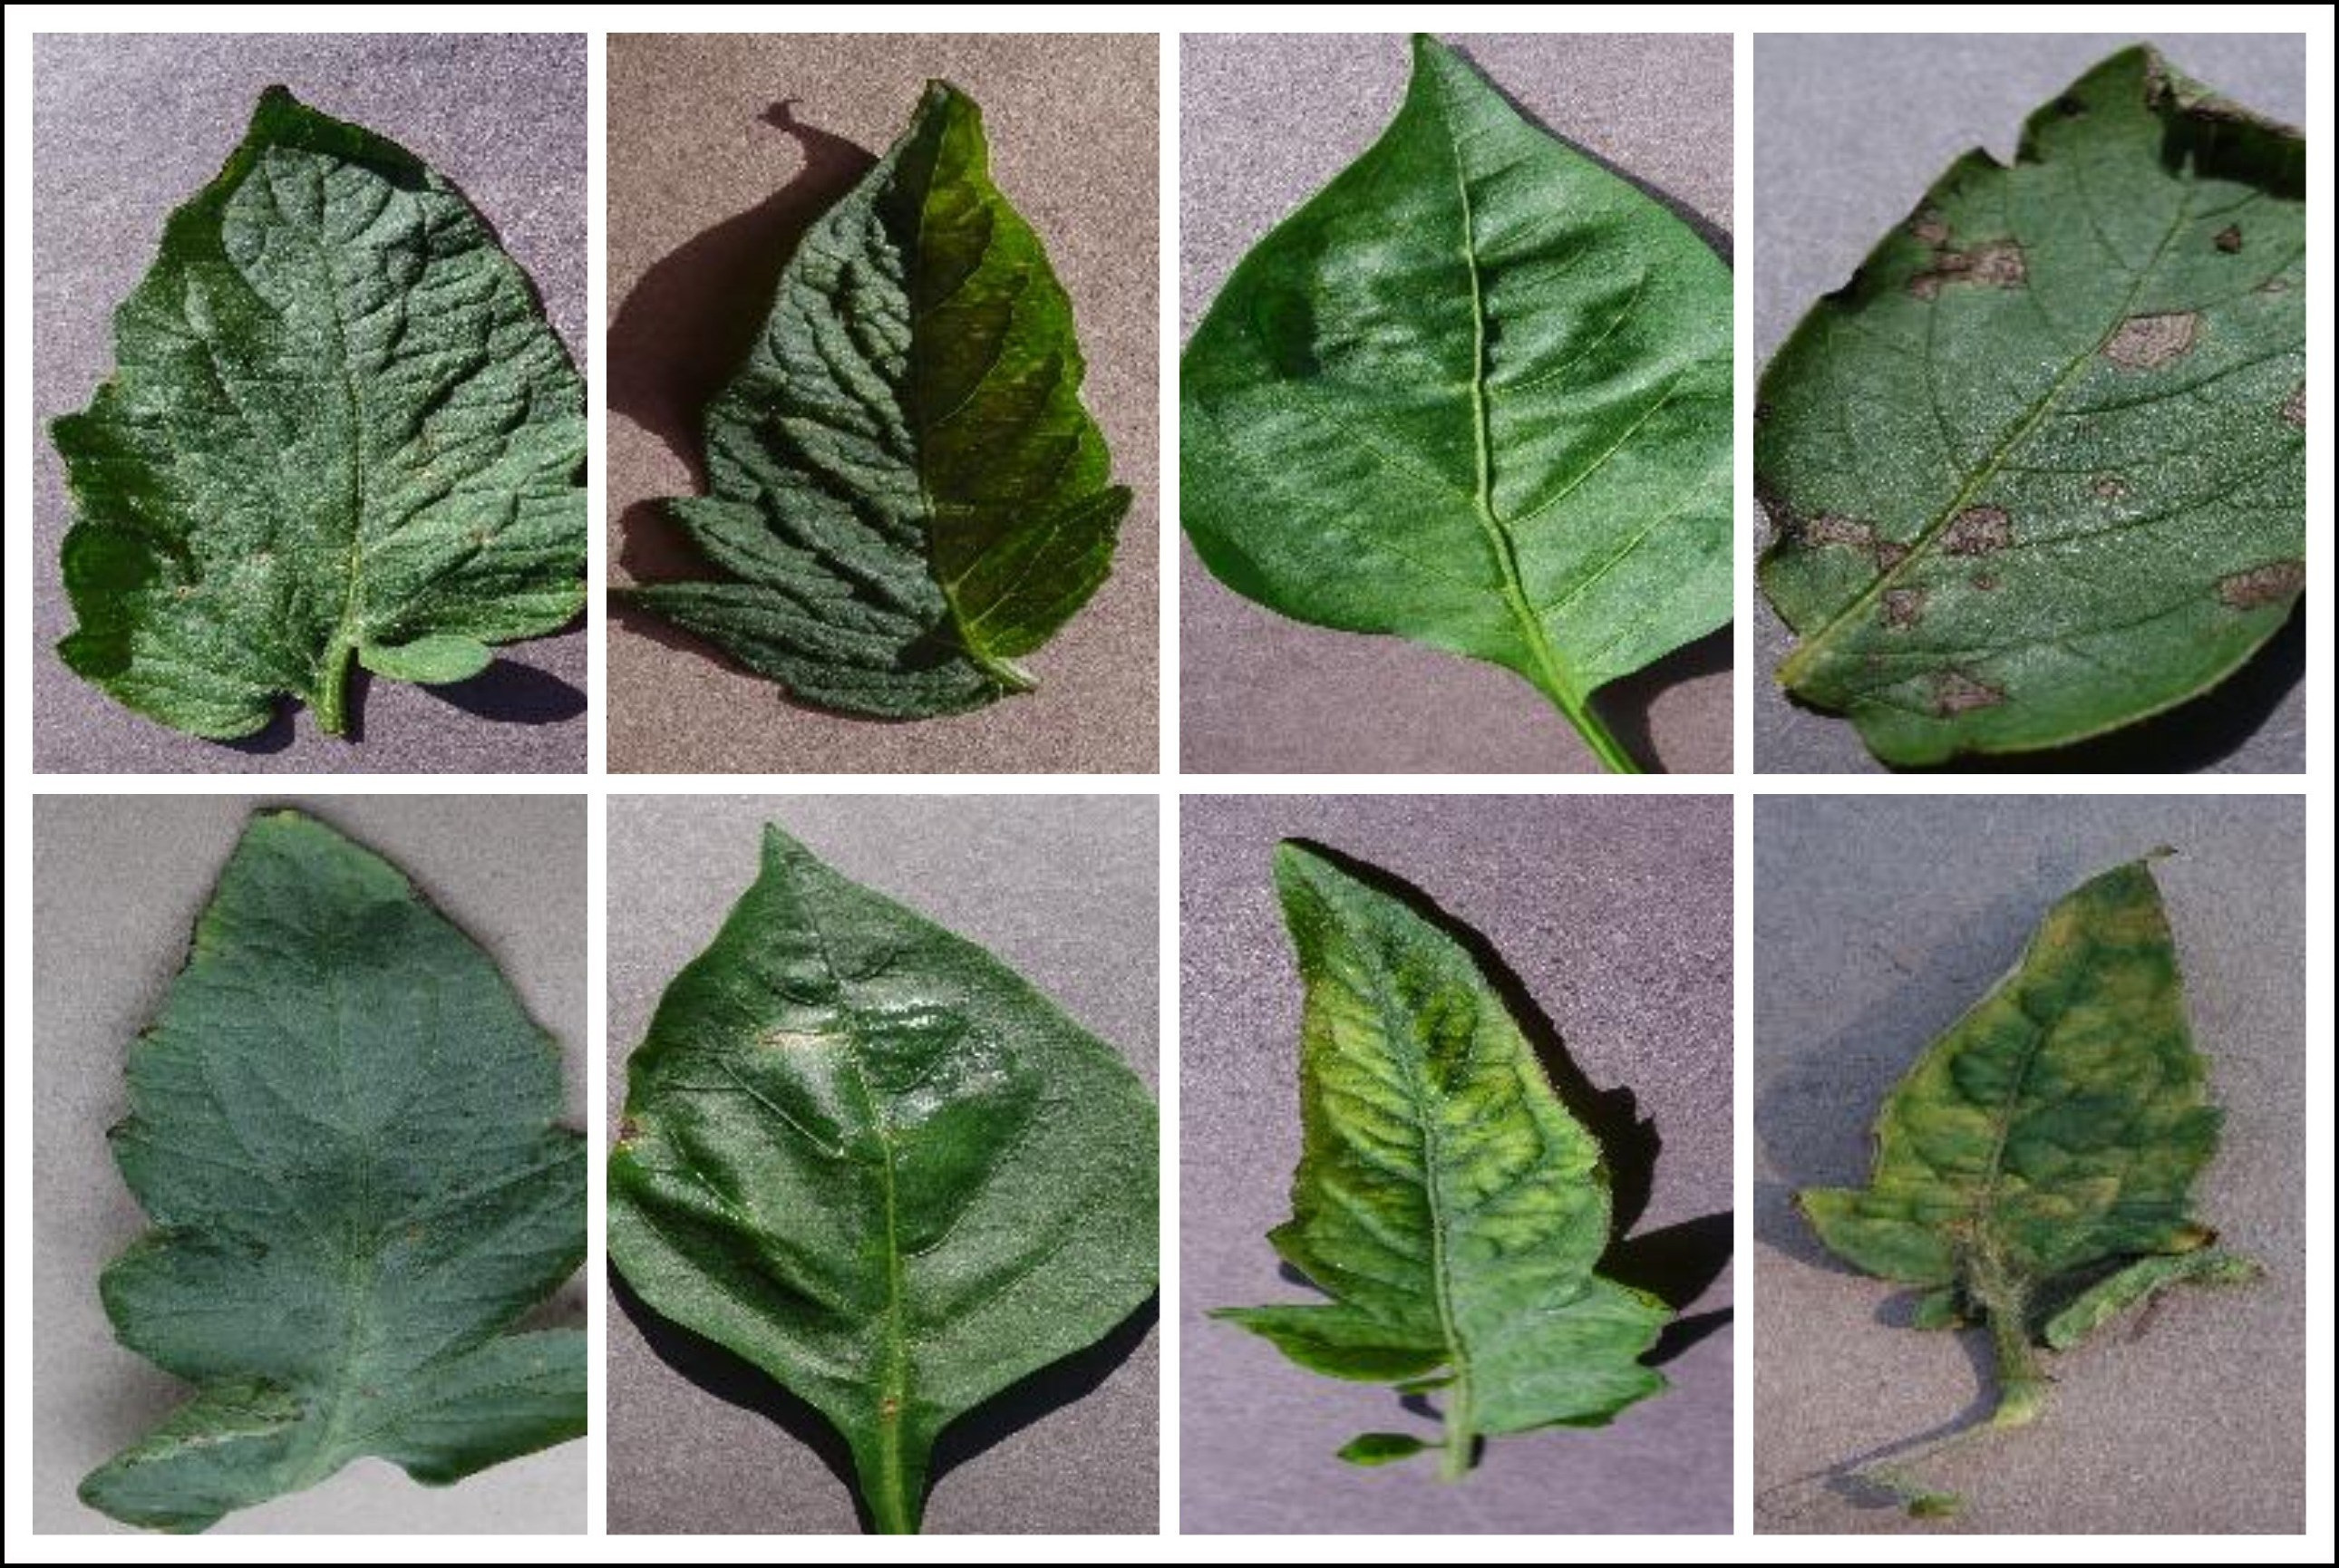
\includegraphics[width=8.8cm, height=5cm]{dataset.jpg}
\caption{Images from the datasets used}
\label{fig: Figure 2}
\end{figure}
 
\subsection{Evaluation Measure}
The performance of the recommended CNN model in identifying diseases in tomato, potato, and bell pepper plant leaves was evaluated using several evaluation metrics, with classification accuracy being the primary measure. This measure represents the percentage of correctly identified images in the test set compared to the total number of images.\\ 


In addition to accuracy, a variety of metrics such as recall, precision, and F1-score are employed to evaluate the effectiveness of the suggested model. Precision measures the proportion of correctly predicted positive instances out of all the instances predicted as positive, while recall measures the proportion of correctly predicted positive instances out of all the actual positive instances. The F1-score, a comprehensive metric, calculates the harmonic mean of precision and recall.\
These assessment criteria can be utilized together to evaluate the ability of the proposed CNN model to distinguish between different diseases in tomato, potato, and bell pepper plant leaves. They can also be used to compare the proposed CNN model to other existing models that are currently in use.

\subsection{Experiment setting} 
The proposed CNN model for identifying leaf diseases in tomato, potato, and bell pepper plants is implemented using Python and various libraries, including TensorFlow, Keras, and OpenCV. The model is executed on a computer system equipped with an i7-6800 CPU running at a clock speed of 3.4 GHz, a 2 GB NVIDIA GeForce GPU, and 16 GB of RAM. Training the model involves using the Adaptive Moment Estimation optimizer for 10 epochs, with a learning rate of 0.001 and a batch size of 128. The dataset of combined tomato, potato, and bell pepper leaf images is divided into three sets: a training set, a validation set, and a testing set, with relative proportions of 70\%, 15\%, and 15\% respectively.


\section{Results and Discussion}
% In this section, we present and discuss the experimental results obtained 

A number of measures, including the F1-score, recall, accuracy, precision, and confusion matrix, were used to evaluate the model's performance. The maximum reported validation accuracy was 95.7\%, whereas the accuracy during training was 93.4\%. The model regularly showed a validation accuracy of 95\%, demonstrating its efficiency in carrying out categorization tasks.

 \begin{figure}[H]
 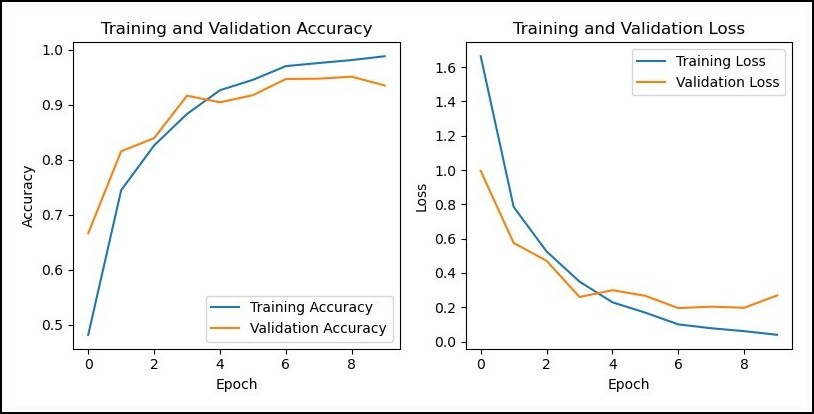
\includegraphics[width=8.9cm, height=4.5cm]{accuracy.jpg}
\caption{The model's accuracy  and loss was assessed during both the training and validation stages.}
\label{fig: Figure 3}
\end{figure}

The accuracy and loss of the model were visualized through graphs. The loss graph demonstrated a gradual decrease in loss followed by a plateau, while the accuracy graph, depicted in Figure~\ref{fig: Figure 3}, exhibited a steady improvement in accuracy before reaching a stable level. These graphs serve as visual evidence of the model's effectiveness and its potential as a valuable tool for classifying the ten different types of tomato leaf diseases. By providing a clear depiction of the model's progress, these graphs enhance our understanding of its capabilities and reinforce its reliability in disease classification.


 \begin{figure}[H]
 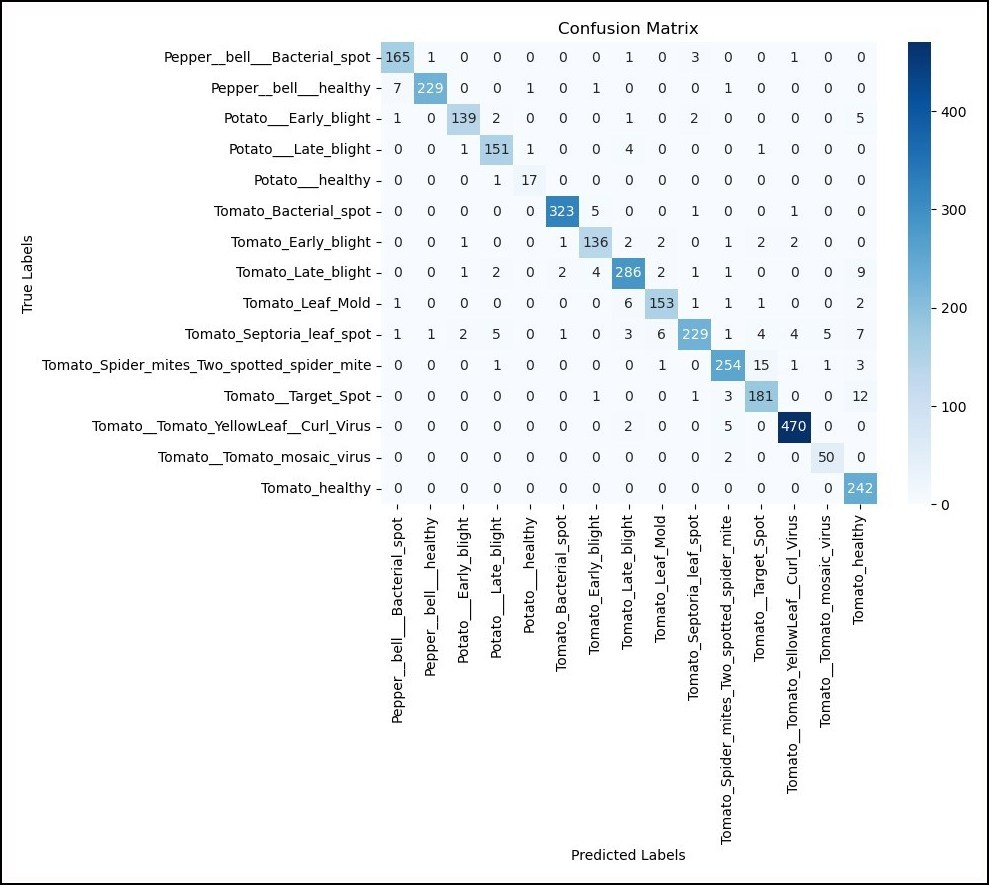
\includegraphics[width=8.8cm, height=5cm]{confusion.jpg}
\caption{Confusion matrix for the model used in the paper}
\label{fig: Figure 4}
\end{figure}

 \begin{figure}[H]
 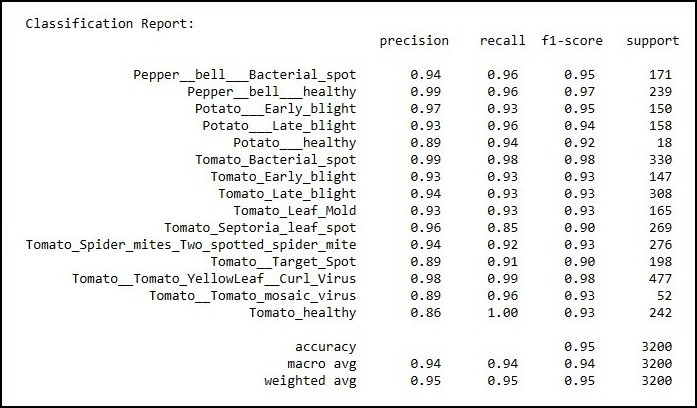
\includegraphics[width=8.8cm, height=4cm]{stats.jpg}
\caption{Accuracy, Precision, Recall and F1-Score for the used model}
\label{fig: Figure 5}
\end{figure}

The performance of image classification models was thoroughly assessed using various metrics, including the confusion matrix, accuracy, precision, recall, and F1 score. The confusion matrix provided a visual representation of the model's performance by comparing the predicted labels with the actual labels. Accuracy was calculated based on the confusion matrix and served as an overall measure of the classification's correctness. The F1 score, shown in figure~\ref{fig: Figure 4}, took into account the model's balance between recall and accuracy. Recall assessed the model's ability to correctly identify positive cases, while precision evaluated its capability to accurately identify all positive instances, as illustrated in figure~\ref{fig: Figure 5}. These evaluations provided comprehensive insights into the model's performance and its ability to classify images effectively.

  
\section{Conclusion and Future Work}
For India's agricultural industry, which is crucial in providing for a sizeable section of the population, to continue to grow sustainably, effective crop disease detection is crucial. Similar to tomatoes, potatoes are prone to a number of illnesses that can have a negative influence on their growth and output. Using the Plant Village dataset, this study proposes a simple method for recognising and diagnosing illnesses in potato leaves using a convolutional neural network (CNN) model. The model uses only a little amount of computer resources to reach outstanding levels of accuracy, ranging from 93\% to 95\%, by examining leaf pictures and finding patterns and traits. The use of data augmentation techniques significantly improves the model's performance and resilience. Alternative optimizers, learning rates, and innovative designs can all be investigated in next research to further improve the model's performance. Optimising the training settings might also assist shorten the training period. This approach is not just applicable to potatoes; it may also be used to identify diseases in other plants, including apples and cucumbers.



% \section*{Acknowledgment}
% This work is supported by the FIST project of Department of Science and Technology, Govt. of India. We thank Mr. xxxxxxxxxxxxxxxxxx for his assistance with language editing, and proofreading. 
%\section{References}
\bibliographystyle{IEEEtran}
\bibliography{santos_bib}

\end{document}







